\section{Generalized Broyden tridiagonal function}
\label{sec:generalized_broyden_results}

The generalized Broyden tridiagonal function is defined as follows.
\begin{align}
F(x) &= \frac12 \sum_{i=1}^n f_k^2(x) &
f_k(x) &= (3-2x_k)x_k + 1 - x_{k-1} - x_{k+1}
\end{align}
Figure \ref{fig:generalized_broyden_surf} shows the surface plot of the 2-dimensional generalized Broyden tridiagonal function.
Notice that the area where the minimum lies is very flat, which makes it hard to converge to the minimum.

\begin{figure}
    \centering
    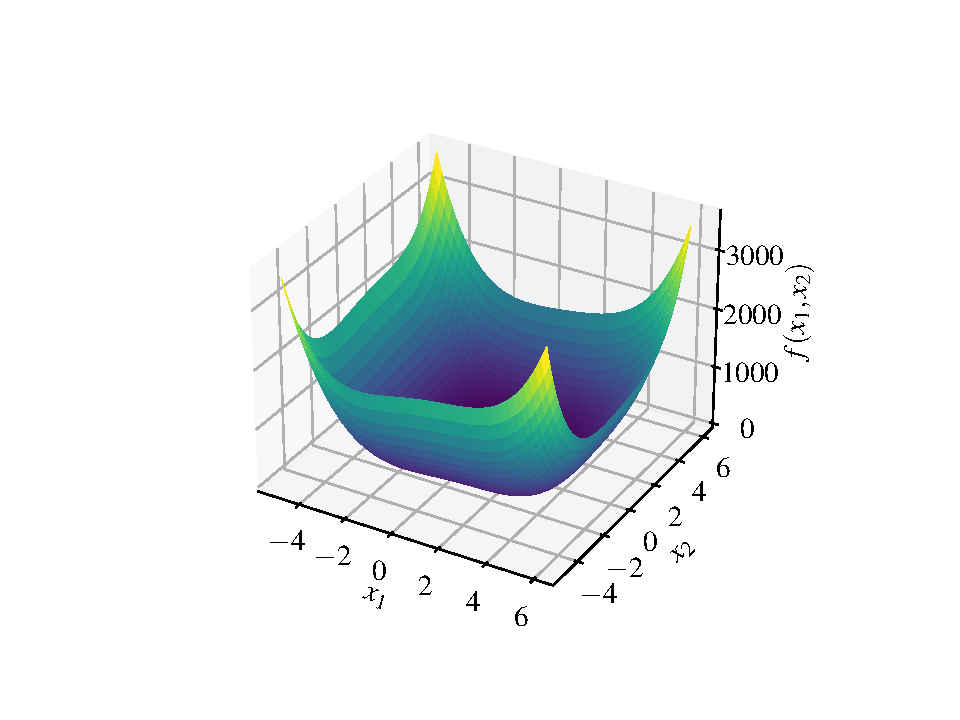
\includegraphics[width=0.5\textwidth]{figures/generalized_broyden_surf.pdf}
    \caption{Surface plot of the 2-dimensional generalized Broyden tridiagonal function}
    \label{fig:generalized_broyden_surf}
\end{figure}

\subsection{Exact gradient and Hessian}

The gradient of the generalized Broyden tridiagonal function is given by the following expression,
\begin{equation}
    \frac{\partial F}{\partial x_k} = \left \{ \begin{array}{ll}
    (3 - 4x_1)f_1(x) - f_2(x), & k = 1\\
    (3-4x_k)f_k(x) - f_{k+1}(x) - f_{k-1}(x), & 1 < k < n\\
    (3-4x_n)f_n(x) - f_{n-1}, & k = n
    \end{array} \right .
\end{equation}
computation can be eased considering that component $k$ depends only on $f_k$, $f_{k+1}$ and $f_{k-1}$.
The Hessian of the generalized Broyden tridiagonal function is given by the following expression.
\begin{equation}
    \frac{\partial^2 F}{\partial x_k \partial x_j} = \left \{ \begin{array}{ll}
    (3-4x_1)^2 - 4f_1(x) + 1, & k = j = 1 \\
    (3-4x_k)^2 - 4f_k(x) + 2, & 1 < k = j < n\\
    (3-4x_n)^2 - 4f_n(x) + 1, & k = j = n \\
    4x_k + 4x_{k+1} - 6, & |k-j| = 1\\
    1, & |k-j| = 2\\
    0, & \text{otherwise}
    \end{array} \right .
\end{equation}
Notice that the Hessian is a banded matrix, with only $n$ non-zero elements on the diagonal, $n-1$ non-zero elements on the first co-diagonal and $n-2$ non-zero elements on the second codiagonal.

Table \ref{tab:Modified_Newton_Generalized_Broyden_exact} shows the results for the \textit{Modified Newton method} applied to the generalized Broyden tridiagonal function with exact gradient and Hessian.
All attempts are succesful, and the method converges in a small number of iterations.
Convergence rate is close to 2, which is the expected convergence rate for Newton's method.
Preconditioning does not seem to have a significant impact on the performance of the method, compared to its impact on the performance on the extended Rosenbrock function due to the fact that the Hessian matrix for the Newton system is better scaled in the currently considered function.

Table \ref{tab:Truncated_Newton_Generalized_Broyden_exact} shows the results for the \textit{Truncated Newton method} applied to the generalized Broyden tridiagonal function with exact gradient and Hessian.
All attempts are succesful, and the method converges in a small number of iterations.
When preconditioning is not adopted convergence rate is lower than 2, which is expected since we are solving the Newton system with a relative tolerance that is guaranteed to yield superlinear convergence.
Differently from the Modified Newton method, the Truncated Newton method is more sensitive to preconditioning, which can be observed by the fact that the number of iterations is lower when preconditioning is adopted and convergence rate is almost 2.

Comparing performance of the two methods, the Truncated Newton method is 2 to 3 times faster than the Modified Newton method due to the fact that the Newton system is solved approximately, which is less computationally expensive than solving it exactly.
However, the Truncated Newton methods requires more iterations to converge than the Modified Newton method, which is expected since the Modified Newton exactly solves the Newton system at each iteration.

\begin{table}
\centering
\caption{Results for Modified Newton method applied to Generalized Broyden with exact gradient and hessian, metrics are average metrics for succesful attempts.}
\label{tab:Modified_Newton_Generalized_Broyden_exact}
\begin{tabular}{r|cc|cc|cc|cc}
\toprule
    & \multicolumn{2}{|c}{iterations} & \multicolumn{2}{|c}{convergence rate} & \multicolumn{2}{|c}{time} & \multicolumn{2}{|c}{success rate} \\
preconditioning & False & True & False & True & False & True & False & True \\
dimension &  &  &  &  &  &  &  &  \\
\midrule
3 & 8.636 & 8.636 & 1.974 & 1.978 & 0.006 & 0.005 & 1.00 & 1.00 \\
4 & 8.000 & 8.273 & 1.829 & 1.849 & 0.037 & 0.034 & 1.00 & 1.00 \\
5 & 7.909 & 10.545 & 1.794 & 1.989 & 0.291 & 0.300 & 1.00 & 1.00 \\
\bottomrule
\end{tabular}
\end{table}

\begin{table}
\centering
\caption{Results for Truncated Newton method applied to Generalized Broyden with exact gradient and hessian, metrics are average metrics for succesful attempts.}
\label{tab:Truncated_Newton_Generalized_Broyden_exact}
\begin{tabular}{r|cc|cc|cc|cc}
\toprule
    & \multicolumn{2}{|c}{iterations} & \multicolumn{2}{|c}{convergence rate} & \multicolumn{2}{|c}{time} & \multicolumn{2}{|c}{success rate} \\
preconditioning & False & True & False & True & False & True & False & True \\
dimension &  &  &  &  &  &  &  &  \\
\midrule
3 & 11.818 & 9.000 & 1.774 & 1.971 & 0.002 & 0.003 & 1.00 & 1.00 \\
4 & 12.727 & 9.727 & 1.346 & 1.987 & 0.014 & 0.015 & 1.00 & 1.00 \\
5 & 13.727 & 9.636 & 1.905 & 1.923 & 0.125 & 0.108 & 1.00 & 1.00 \\
\bottomrule
\end{tabular}
\end{table}

\subsection{Finite differences gradient and Hessian}

When applying \ref{eq:findiff_gradient}, one can notice that the terms $F(x + he_k)$ and $F(x-he_k)$ only differ by terms $f_k$, $f_{k+1}$ and $f_{k-1}$.
Then to make function evaluations less expensive, we can define the following function $F_{\textit{fd},\,k}$, which can be plugged in \ref{eq:findiff_gradient} in place of $F$ yielding the same result.
\[
F_{\textit{fd},\,k}(x) = \frac12 f_k^2(x) + \frac12 f_{k+1}^2(x) + \frac12 f_{k-1}^2(x)
\]
The same procedure can be applied for the Hessian, considering that:
\begin{itemize}
    \item function evaluations to compute entry $h_{k,k}$ differ only by $f_k$, $f_{k+1}$ and $f_{k-1}$;
    \item function evaluations to compute entry $h_{k,k+1}$ differ only by $f_k$ and $f_{k+1}$;
    \item function evaluations to compute entry $h_{k,k+2}$ differ only by $f_{k-1}$.
\end{itemize}
Then to make function evaluations less expensive, we can define the functions $F_{\textit{fd},\,k,k}$, $F_{\textit{fd},\,k,k+1}$, $F_{\textit{fd},\,k,k+2}$, which can be plugged in \ref{eq:findiff_hessian} in place of $F$ yielding the same result to compute entries $h_{k,k}$, $h_{k,k+1}$ and $h_{k,k+2}$ respectively.
\begin{align*}
F_{\textit{fd},\,k,k}(x) &= \frac12 f_k^2(x) + \frac12 f_{k-1}^2(x) + \frac12 f_{k+1}^2(x)\\
F_{\textit{fd},\,k,k+1}(x) &= \frac12 f_k^2(x) + \frac12 f_{k+1}^2(x)\\
F_{\textit{fd},\,k,k+2}(x) &= \frac12 f_{k-1}^2(x)
\end{align*}
When plugging the functions $F_{fd,\,k}$, $F_{fd,\,k,k}$, $F_{\textit{fd},\,k,k+1}$ and $F_{\textit{fd},\,k,k+2}$ into \ref{eq:findiff_gradient} and \ref{eq:findiff_hessian} it's convenient to expand them so that the computation of the gradient and Hessian is not subject to numerical cancellation as previously done for the extended Rosenbrock function in subsection \ref{subsec:extended_rosenbrock_findiff}.

Tables \ref{tab:Modified_Newton_Generalized_Broyden_fd_abs} and \ref{tab:Modified_Newton_Generalized_Broyden_fd_rel} show the results for the \textit{Modified Newton method} applied to the generalized Broyden tridiagonal function with absolute and specific finite differences respectively.
All attempts are succesful, but attempts with $h=10^{-2}$ which don't converge within the fixed maximum number of iterations $k_{\textit{max}}=1000$, both for absolute and specific differences, for all dimensions.
This is probably due to the fact that $h=10^{-2}$ is not a suitable increment for the finite differences method to approximate the gradient and Hessian of the generalized Broyden tridiagonal function.
When the method converges, it does so in a small number of iterations with a convergence rate close to 2, which is the expected convergence rate for Newton's method.

\begin{table}
\centering
\caption{Results for Modified Newton method applied to Generalized Broyden with absolute finite differences, metrics are average metrics for succesful attempts.}
\label{tab:Modified_Newton_Generalized_Broyden_fd_abs}
\begin{tabular}{rr|cc|cc|cc|cc}
\toprule
    &  & \multicolumn{2}{|c}{iterations} & \multicolumn{2}{|c}{convergence rate} & \multicolumn{2}{|c}{time} & \multicolumn{2}{|c}{success rate} \\
    & preconditioning & False & True & False & True & False & True & False & True \\
dimension & h &  &  &  &  &  &  &  &  \\
\midrule
\multirow[t]{5}{*}{3} & 1e-04 & 8.545 & 8.545 & 2.016 & 2.010 & 0.006 & 0.006 & 1.00 & 1.00 \\
    & 1e-06 & 8.545 & 8.636 & 1.964 & 1.979 & 0.006 & 0.006 & 1.00 & 1.00 \\
    & 1e-08 & 8.636 & 8.636 & 1.974 & 1.978 & 0.006 & 0.005 & 1.00 & 1.00 \\
    & 1e-10 & 8.636 & 8.636 & 1.974 & 1.978 & 0.006 & 0.006 & 1.00 & 1.00 \\
    & 1e-12 & 8.636 & 8.636 & 1.973 & 1.978 & 0.006 & 0.006 & 1.00 & 1.00 \\
\cline{1-10}
\multirow[t]{5}{*}{4} & 1e-04 & 7.909 & 8.273 & 1.803 & 1.829 & 0.036 & 0.031 & 1.00 & 1.00 \\
    & 1e-06 & 8.000 & 8.273 & 1.832 & 1.851 & 0.036 & 0.031 & 1.00 & 1.00 \\
    & 1e-08 & 8.000 & 8.273 & 1.829 & 1.849 & 0.038 & 0.031 & 1.00 & 1.00 \\
    & 1e-10 & 8.000 & 8.273 & 1.829 & 1.849 & 0.038 & 0.031 & 1.00 & 1.00 \\
    & 1e-12 & 8.000 & 8.273 & 1.829 & 1.849 & 0.038 & 0.032 & 1.00 & 1.00 \\
\cline{1-10}
\multirow[t]{5}{*}{5} & 1e-04 & 7.818 & 10.455 & 1.751 & 2.045 & 0.321 & 0.344 & 1.00 & 1.00 \\
    & 1e-06 & 7.909 & 10.545 & 1.796 & 1.992 & 0.333 & 0.332 & 1.00 & 1.00 \\
    & 1e-08 & 7.909 & 10.545 & 1.794 & 1.989 & 0.324 & 0.337 & 1.00 & 1.00 \\
    & 1e-10 & 7.909 & 10.545 & 1.794 & 1.989 & 0.314 & 0.325 & 1.00 & 1.00 \\
    & 1e-12 & 7.909 & 10.545 & 1.794 & 1.989 & 0.320 & 0.328 & 1.00 & 1.00 \\
\cline{1-10}
\bottomrule
\end{tabular}
\end{table}

\begin{table}
\centering
\caption{Results for Modified Newton method applied to Generalized Broyden with specific finite differences, metrics are average metrics for succesful attempts.}
\label{tab:Modified_Newton_Generalized_Broyden_fd_rel}
\begin{tabular}{rr|cc|cc|cc|cc}
\toprule
    &  & \multicolumn{2}{|c}{iterations} & \multicolumn{2}{|c}{convergence rate} & \multicolumn{2}{|c}{time} & \multicolumn{2}{|c}{success rate} \\
    & preconditioning & False & True & False & True & False & True & False & True \\
dimension & h &  &  &  &  &  &  &  &  \\
\midrule
\multirow[t]{5}{*}{3} & 1e-04 & 8.545 & 8.636 & 1.977 & 2.000 & 0.006 & 0.006 & 1.00 & 1.00 \\
    & 1e-06 & 8.545 & 8.636 & 1.964 & 1.979 & 0.006 & 0.005 & 1.00 & 1.00 \\
    & 1e-08 & 8.636 & 8.636 & 1.974 & 1.978 & 0.007 & 0.007 & 1.00 & 1.00 \\
    & 1e-10 & 8.636 & 8.636 & 1.973 & 1.978 & 0.006 & 0.006 & 1.00 & 1.00 \\
    & 1e-12 & 8.636 & 8.636 & 1.973 & 1.978 & 0.007 & 0.006 & 1.00 & 1.00 \\
\cline{1-10}
\multirow[t]{5}{*}{4} & 1e-04 & 7.909 & 8.273 & 1.804 & 1.835 & 0.037 & 0.031 & 1.00 & 1.00 \\
    & 1e-06 & 8.000 & 8.273 & 1.830 & 1.850 & 0.050 & 0.031 & 1.00 & 1.00 \\
    & 1e-08 & 8.000 & 8.273 & 1.829 & 1.849 & 0.038 & 0.032 & 1.00 & 1.00 \\
    & 1e-10 & 8.000 & 8.273 & 1.829 & 1.849 & 0.038 & 0.032 & 1.00 & 1.00 \\
    & 1e-12 & 8.000 & 8.273 & 1.829 & 1.849 & 0.038 & 0.031 & 1.00 & 1.00 \\
\cline{1-10}
\multirow[t]{5}{*}{5} & 1e-04 & 7.818 & 10.545 & 1.752 & 2.020 & 0.315 & 0.325 & 1.00 & 1.00 \\
    & 1e-06 & 7.909 & 10.545 & 1.795 & 1.990 & 0.314 & 0.326 & 1.00 & 1.00 \\
    & 1e-08 & 7.909 & 10.545 & 1.794 & 1.989 & 0.329 & 0.329 & 1.00 & 1.00 \\
    & 1e-10 & 7.909 & 10.545 & 1.794 & 1.989 & 0.325 & 0.327 & 1.00 & 1.00 \\
    & 1e-12 & 7.909 & 10.545 & 1.794 & 1.989 & 0.313 & 0.325 & 1.00 & 1.00 \\
\cline{1-10}
\bottomrule
\end{tabular}
\end{table}

Tables \ref{tab:Truncated_Newton_Generalized_Broyden_fd_abs} and \ref{tab:Truncated_Newton_Generalized_Broyden_fd_rel} show the results for the \textit{Truncated Newton method} applied to the generalized Broyden tridiagonal function with absolute and specific finite differences respectively.
All attempts are succesful, but attempts with $h=10^{-2}$ which converge within the fixed maximum number of iterations $k_{\textit{max}}=1000$ only once for $n=10^3$, regardless of the type (absolute or specific) of finite differences adopted.
When the method converges, it does so in a small number of iterations with a convergence rate that as expected is superlinear, almost quadratic for $n = 10^5$, even if preconditioning is not adopted. 
When preconditioning is adopted, the number of iterations is lower and the convergence rate is closer to 2, which is the expected convergence rate for Newton's method.

Also for this function, it's evident that the Truncated Newton method is faster than the Modified Newton method, but requires more iterations to converge.
Moreover, the Truncated Newton method is more sensitive to preconditioning than the Modified Newton method.
    
\begin{table}
\centering
\caption{Results for Truncated Newton method applied to Generalized Broyden with absolute finite differences, metrics are average metrics for succesful attempts.}
\label{tab:Truncated_Newton_Generalized_Broyden_fd_abs}
\begin{tabular}{rr|cc|cc|cc|cc}
\toprule
    &  & \multicolumn{2}{|c}{iterations} & \multicolumn{2}{|c}{convergence rate} & \multicolumn{2}{|c}{time} & \multicolumn{2}{|c}{success rate} \\
    & preconditioning & False & True & False & True & False & True & False & True \\
dimension & h &  &  &  &  &  &  &  &  \\
\midrule
\multirow[t]{6}{*}{3} & 1e-02 & 13.000 & NaN & 1.051 & NaN & 0.002 & NaN & 0.09 & NaN \\
    & 1e-04 & 11.818 & 9.091 & 1.773 & 2.009 & 0.003 & 0.003 & 1.00 & 1.00 \\
    & 1e-06 & 11.818 & 9.000 & 1.774 & 1.972 & 0.003 & 0.003 & 1.00 & 1.00 \\
    & 1e-08 & 11.818 & 9.000 & 1.774 & 1.971 & 0.003 & 0.003 & 1.00 & 1.00 \\
    & 1e-10 & 11.818 & 9.000 & 1.774 & 1.971 & 0.003 & 0.003 & 1.00 & 1.00 \\
    & 1e-12 & 11.818 & 9.000 & 1.774 & 1.971 & 0.003 & 0.004 & 1.00 & 1.00 \\
\cline{1-10}
\multirow[t]{5}{*}{4} & 1e-04 & 12.727 & 9.545 & 1.347 & 1.995 & 0.019 & 0.018 & 1.00 & 1.00 \\
    & 1e-06 & 12.727 & 9.727 & 1.346 & 1.990 & 0.018 & 0.017 & 1.00 & 1.00 \\
    & 1e-08 & 12.727 & 9.727 & 1.346 & 1.987 & 0.018 & 0.017 & 1.00 & 1.00 \\
    & 1e-10 & 12.727 & 9.727 & 1.346 & 1.987 & 0.018 & 0.018 & 1.00 & 1.00 \\
    & 1e-12 & 12.727 & 9.727 & 1.346 & 1.987 & 0.019 & 0.018 & 1.00 & 1.00 \\
\cline{1-10}
\multirow[t]{5}{*}{5} & 1e-04 & 13.727 & 9.545 & 1.905 & 1.903 & 0.160 & 0.132 & 1.00 & 1.00 \\
    & 1e-06 & 13.727 & 9.636 & 1.905 & 1.926 & 0.162 & 0.133 & 1.00 & 1.00 \\
    & 1e-08 & 13.727 & 9.636 & 1.905 & 1.923 & 0.159 & 0.137 & 1.00 & 1.00 \\
    & 1e-10 & 13.727 & 9.636 & 1.905 & 1.923 & 0.161 & 0.132 & 1.00 & 1.00 \\
    & 1e-12 & 13.727 & 9.636 & 1.905 & 1.923 & 0.156 & 0.132 & 1.00 & 1.00 \\
\cline{1-10}
\bottomrule
\end{tabular}
\end{table}

\begin{table}
\centering
\caption{Results for Truncated Newton method applied to Generalized Broyden with specific finite differences, metrics are average metrics for succesful attempts.}
\label{tab:Truncated_Newton_Generalized_Broyden_fd_rel}
\begin{tabular}{rr|cc|cc|cc|cc}
\toprule
    &  & \multicolumn{2}{|c}{iterations} & \multicolumn{2}{|c}{convergence rate} & \multicolumn{2}{|c}{time} & \multicolumn{2}{|c}{success rate} \\
    & preconditioning & False & True & False & True & False & True & False & True \\
dimension & h &  &  &  &  &  &  &  &  \\
\midrule
\multirow[t]{5}{*}{3} & 1e-04 & 11.818 & 9.091 & 1.773 & 1.986 & 0.003 & 0.003 & 1.00 & 1.00 \\
    & 1e-06 & 11.818 & 9.000 & 1.774 & 1.971 & 0.003 & 0.003 & 1.00 & 1.00 \\
    & 1e-08 & 11.818 & 9.000 & 1.774 & 1.971 & 0.003 & 0.003 & 1.00 & 1.00 \\
    & 1e-10 & 11.818 & 9.000 & 1.774 & 1.971 & 0.003 & 0.004 & 1.00 & 1.00 \\
    & 1e-12 & 11.818 & 9.000 & 1.774 & 1.971 & 0.003 & 0.003 & 1.00 & 1.00 \\
\cline{1-10}
\multirow[t]{5}{*}{4} & 1e-04 & 12.727 & 9.545 & 1.347 & 1.982 & 0.018 & 0.017 & 1.00 & 1.00 \\
    & 1e-06 & 12.727 & 9.727 & 1.346 & 1.989 & 0.017 & 0.018 & 1.00 & 1.00 \\
    & 1e-08 & 12.727 & 9.727 & 1.346 & 1.987 & 0.018 & 0.018 & 1.00 & 1.00 \\
    & 1e-10 & 12.727 & 9.727 & 1.346 & 1.987 & 0.017 & 0.017 & 1.00 & 1.00 \\
    & 1e-12 & 12.727 & 9.727 & 1.346 & 1.987 & 0.018 & 0.018 & 1.00 & 1.00 \\
\cline{1-10}
\multirow[t]{5}{*}{5} & 1e-04 & 13.727 & 9.636 & 1.905 & 1.930 & 0.155 & 0.133 & 1.00 & 1.00 \\
    & 1e-06 & 13.727 & 9.636 & 1.905 & 1.924 & 0.159 & 0.131 & 1.00 & 1.00 \\
    & 1e-08 & 13.727 & 9.636 & 1.905 & 1.923 & 0.160 & 0.134 & 1.00 & 1.00 \\
    & 1e-10 & 13.727 & 9.636 & 1.905 & 1.923 & 0.158 & 0.132 & 1.00 & 1.00 \\
    & 1e-12 & 13.727 & 9.636 & 1.905 & 1.923 & 0.156 & 0.132 & 1.00 & 1.00 \\
\cline{1-10}
\bottomrule
\end{tabular}
\end{table}